%!TEX root = ../main/main.tex
\newpage

\section{Deployment View} % (fold)
\label{sec:deployment_view}

In this section we analyze the \emph{Deployment View}, meaning that a presentation of the deployment point of view is provided.

\subsection{Diagram} % (fold)
\label{ssub:diagram}

In order to have a successful deployment an in depth analysis of the main components that will have to be deployed is required.

For this reason here is a diagram showing the \emph{Deployment View}:

\begin{figure}[h!t]
\caption{Deployment Diagram}
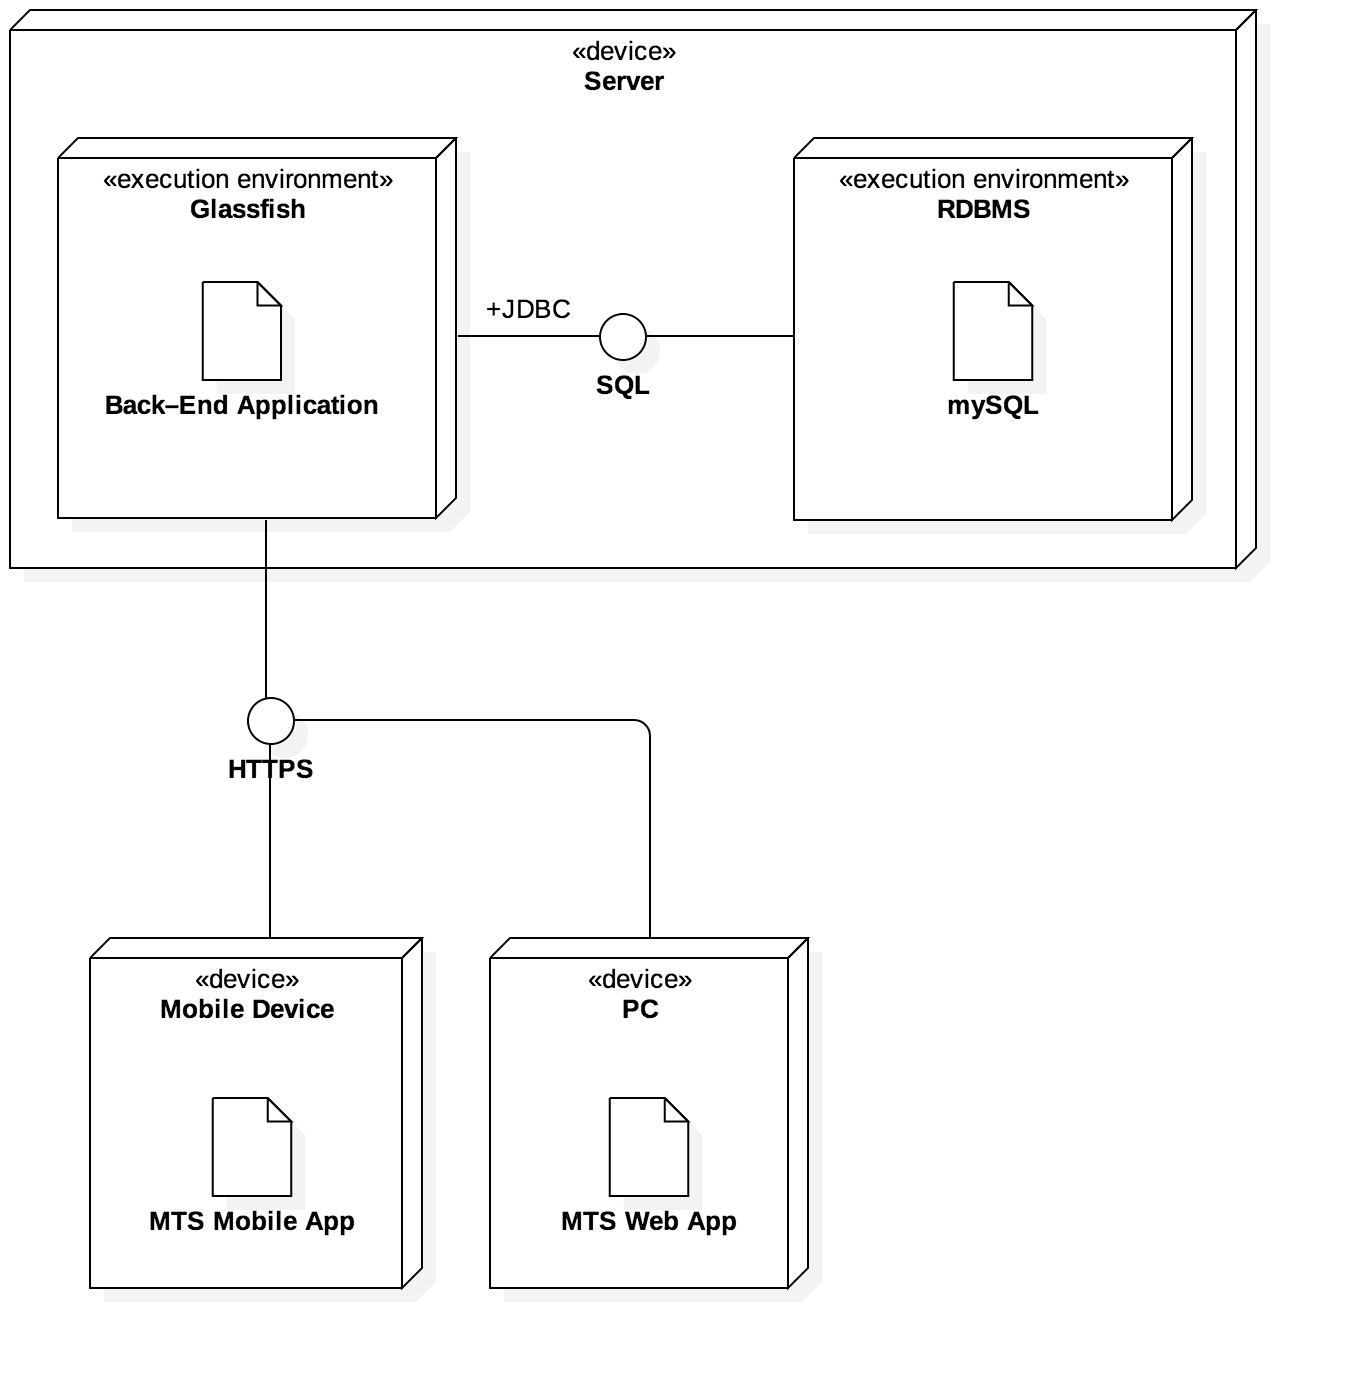
\includegraphics[width=\textwidth]{diagram/png/DeploymentDiagram}
\centering
\end{figure}
\newpage

% subsubsection diagram (end)

\subsection{Diagram Analysis} % (fold)
\label{ssub:diagram_analysis}

% subsubsection diagram_analysis (end)
This diagram shows a two-tier architecture.

A main server is deployed: in this node the \emph{mySQL DataBase} is executed. This is also where the \emph{Back-End Application} will be deployed.

Both mobile applications, the \emph{User} one and the \emph{Taxi Driver} one, interface with the \emph{\nameref{par:back_end_application}} through \emph{HTTP} protocol.
Also the PC application, namely the \emph{Web Application}, connects to \emph{\nameref{par:back_end_application}}.
% section deployment_view (end)